% !TEX encoding = Windows Latin 1
\documentclass{llncs}
\usepackage{graphicx}
\usepackage[english]{babel}
\usepackage{color}
\usepackage{ucs}
\usepackage[latin1]{inputenc}

\newcommand{\markus}[1]{\textcolor{red}{Markus: #1}}
\newcommand{\arif}[1]{\textcolor{blue}{Arif: #1}}
\newcommand{\lars}[1]{\textcolor{greed}{Lars: #1}}

\renewcommand\floatpagefraction{.9}
\renewcommand\topfraction{.9}
\renewcommand\bottomfraction{.9}
\renewcommand\textfraction{.1}   
\setcounter{totalnumber}{50}
\setcounter{topnumber}{50}
\setcounter{bottomnumber}{50}

\bibliographystyle{splncs03}

\begin{document}
\frontmatter        
\pagestyle{headings}
\mainmatter           

\title{Traces in the Analysis of Heterogenous (Numeric) Data (in SNs)}

\author{Markus Scheidgen}
\authorrunning{M. Scheidgen}
\institute{Department of Computer Science, Humboldt Universit�t zu Berlin\\
           Unter den Linden 6, 10099 Berlin, Germany\\
           \email{\{scheidge\}@informatik.hu-berlin.de}}

\maketitle
%\thispagestyle{empty}

\begin{abstract} 
\markus{TODO}
\end{abstract}

\section{Introduction}\label{sec:introduction}

\subsection{The examples}

All examples in this paper are taken form the domains \emph{wireless mesh networks} (WMN) and \emph{wireless sensor networks} (WSN). Specifically, all example are taken from the \emph{Humboldt Wireless Lab} (HWL) test-bed. The HWL test-bed is a WSN based on WMN technology. Therefore, the HWL test-bed is both a WMN and WNS.

\subsection{The nature of data and information}\label{sec:information}

Terms like data or information are ambiguous and hence have potentially different and confusing means is different communities. \emph{Disclaimer:} The following is not an attempt to provide some sort of commonly accepted information theory; it only serves the cause of this paper.

We start with the smallest pieces: \emph{atomic pieces of data} (APD). APDs do not contain other data but themselves. An APD has an \emph{identity}, \emph{value}, and \emph{data type}. The set of values of all APDs of a certain type form the \emph{defining set} of that data type. Many data types are defined through (subsets) of real or natural numbers, such as temperature values between -30 and 100 degree Celsius. A set of labels is also a typical APD type. But data types are not limited to numbers and strings. Tuples of numbers, bitmaps, graphs, etc can also be the values of APDs, but only if these APDs are never considered to consist of multiple parts. Each APD has an identity. Two APDs from type integer, are not necessarily the same just because their values are equals.

\begin{figure}
  \centering
  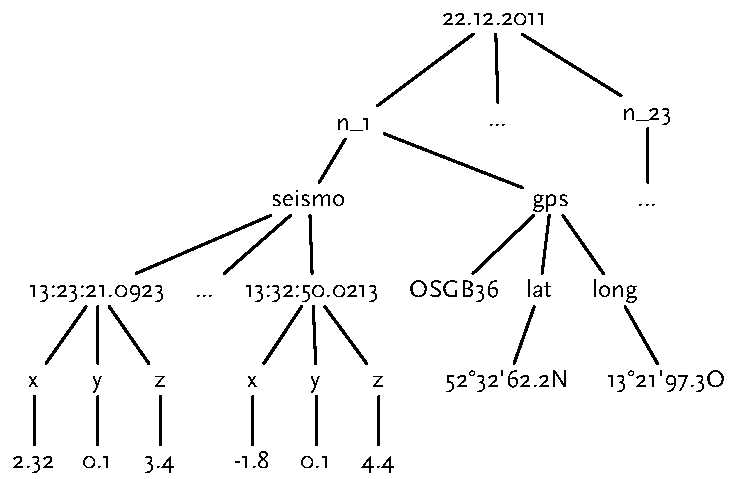
\includegraphics[width=0.65\linewidth]{figures/example_information_graph}
  \caption{Experiment data (information) from the HWL a WMN/WSN with seismo and gps sensors}
  \label{fig:example_information_graph}
\end{figure}

Because each single APD does not have any context, it is considered \emph{data} and not information. But APDs can be linked to each other. We consider graphs of APDs as \emph{information}. The vertices are takes from a set of APDs and edges connect different APDs. In such a graph each APD has a \emph{context}: that are the neighbors of an APD. 

We assume that each information graph contains a designated information tree. 
An \emph{information tree} is a directed and acyclic graph subgraph that covers all vertices (i.e. all APDs). Edges are directed from \emph{child} to \emph{parent}. One child can have multiple parents, one parent can have multiple parents, diamonds are allowed. An information graph can contain multiple information trees, but one tree must be designated and is called \emph{the information (or composite) tree of an information graph}. 

In an information tree edges provide an antisymmetric relationship between APDs. The reflexive transitive hull of this relationship induces a partial order among APDs in an information graph. We simple say an APD is \emph{related} to another APD, iff these APDs are related with respect to this reflexive transitive hull. Note that children are only related to parents and not vice versa. The set of all related APDs of an APD is called \emph{ancestors} of that APD. The joint of ancestors of a set of APDs is called the \emph{common ancestors} of that set. The set of smallest ancestors is called the \emph{closest ancestors} of a set of APDs. Two APDs are \emph{siblings} if they have a non empty set of common ancestors. 

The information graph if Fig.~\ref{fig:example_information_graph} for example comprises of all the data from an experiment with a WSN of 23 nodes and two sensors (seismo and gps). This includes APDs with several types: date, time, node identifiers, sensor identifiers, spatial axis, accelerometer readings, degrees (long/lat), and coordinate reference systems. The ancestors of each accelerometer reading contain a axis, a time, a node, and an experiment date. Each accelerometer reading and each gps coordinate at least share the experiment date as common ancestor. An accelerometer reading and a gps coordinate of the same node share also the node as common ancestor. 

Information has also a type (\emph{information type}). Consider the WSN from the last example: all possible information graphs from experiments with this WSN share a unique structure. There are constraints for the set of possible APDs and possible edges.

There are several technical systems to create, store, and access information. XML files can contain information trees (and graphs) where each entity (or attribute) represents an APD. XML schema define types of information. Relational databases organize information in tables and references between entries of different tables. Each value (specific entry, specific column) in a relational database table is a APD. Entries and relationships form links between APDs. Entity relationship diagrams or database schemas define types of information. Models (as in OMG) are information, objects (and attributes) are APDs. Meta-models define types of information. Within programming languages data structures (classes, structs, union, arrays and primitive types) are used to represent information. Further systems are based on ontologies or RDF.

There are several abstractions for the representation of information. We may call graphs of APDs information, but these graphs are actually only one possible abstraction. Other (somewhat limited) representations are list, maps, functions, terms, different forms of trees and graphs, algebras, vectors, matrices, tables, etc. Of cause different representations can be combined. 

\subsection{Analysis and Traces}
 
\begin{figure}
  \centering
  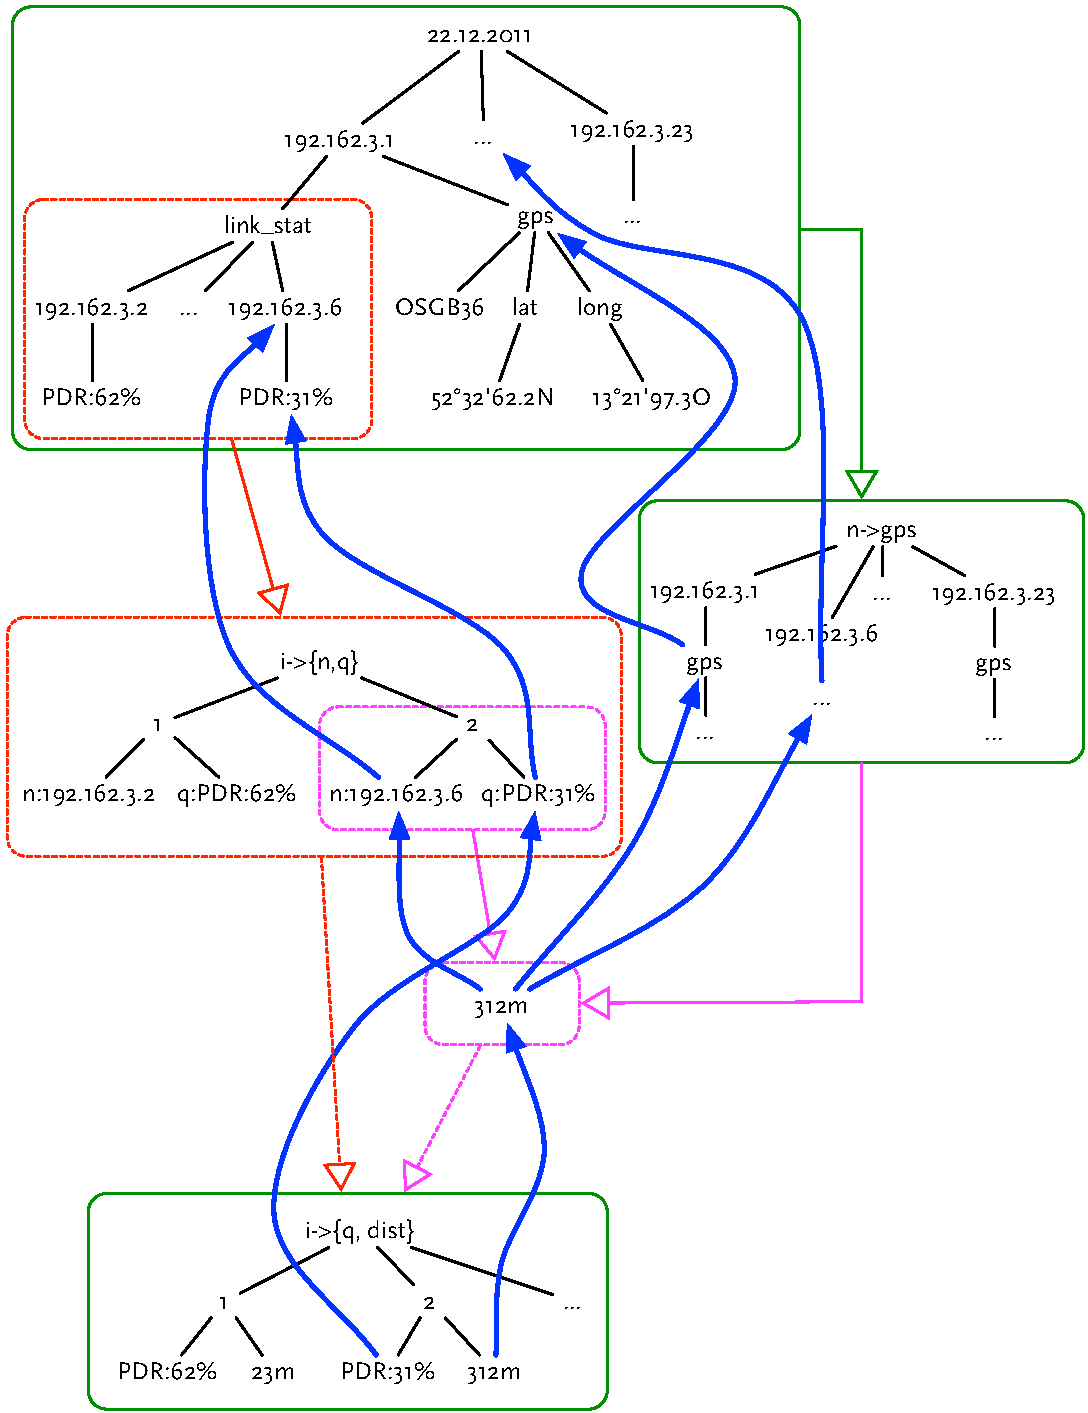
\includegraphics[width=\linewidth]{figures/example_analysis_data}
  \caption{An example for Information in different analysis steps and traces between its APDs. The example is taken from an experiment with the HWL network. The information obtained within the network includes information about links and link quality (packed delivery rate, PDR) and the position of the nodes (via global positioning system, GPS). The colored boxes mark distinct information graphs. The thin colored arrows mark analysis steps, the arrow point marks the created information graph. Green boxes mark information graphs that cover the whole experiment, other colors mark information graphs that only cover single samples. In the example, the red box describe the links of one network node, the purple boxes describe a single link. The thick blue arrows mark traces between APDs: the arrows show which APD is based on what other APDs.}
  \label{fig:example_analysis_data}
\end{figure}

The information graphs considered in this paper (e.g. the information graphs defined and exemplified in section~\ref{sec:information}) are to be analyzed. Information is usually created during experiments. These experiment results are on low level of abstraction and we want to extract information on a higher layer of abstraction. The term \emph{analysis} describes the process in which new information graphs are created from existing information graph. An analysis can be divided into analysis steps. In each \emph{analysis step} a distinct information graph is created. An analysis can have multiple steps and hence produce intermediate information graphs, i.e. intermediate results. Fig.~\ref{fig:example_analysis_data} shows the information graphs of an example analysis.

When a new information graph is created during an analysis step, APDs of the new graph can be assigned to APDs of existing information graphs: new APDs are either directly taken (copy) or are computed from one or more existing APDs. This creates a directed relationship between APDs of different information graphs. This relationship is antisymmetric. The reflexive transitive hull links one APD to all those APD that participate in its creation (including the APD itself). We denote this relation \emph{trance relation}. The trace relation induces a partial order. The ordered set of APDs that participate in the creation of an APD (including the APD itself) is called the \emph{trace} of that APD.

Original information graph, intermediate and final results of an analysis as well as the trace relationship can be used to form a union information graph. The trace relationship and all information trees compose the composition tree of that new information graph. We call this information graph the \emph{analysis information graph} and the original information graph the \emph{experiment information graph}. 

Analysis information graphs can be further extended. Depending on the type and semantic of APDs, we can define (usually equivalence) relationships on the values of APDs. For example: to denote close proximity GPS coordinates can be designated equivalent, timestamps can be designated equivalent if they shell denote the same point in time, etc. This way, two APDs can be \emph{weak siblings} if they share ancestors with different identity but (similar or) same meaning.

\begin{figure}
  \centering
  \parbox{0.45\linewidth}{%
    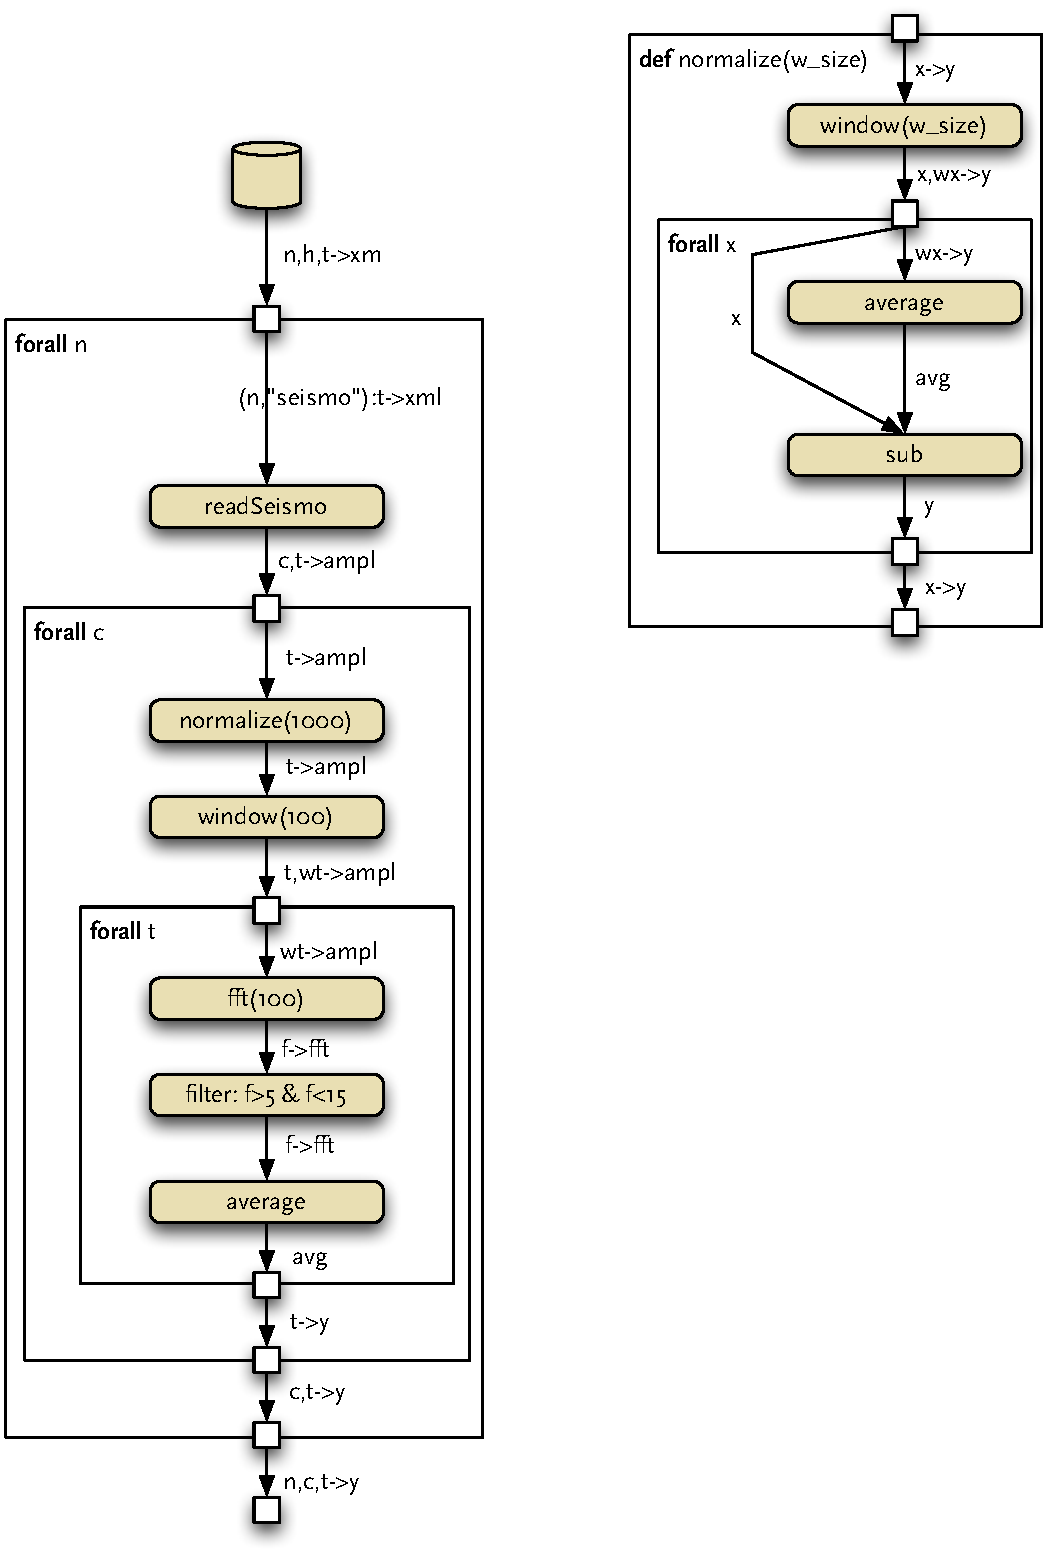
\includegraphics[width=\linewidth]{figures/seismo_bus_composition}
    \caption{Seismo analysis composition.}%
    \label{fig:seismo_bus_composition}
  }%
  \qquad
  \begin{minipage}{0.45\linewidth}%
    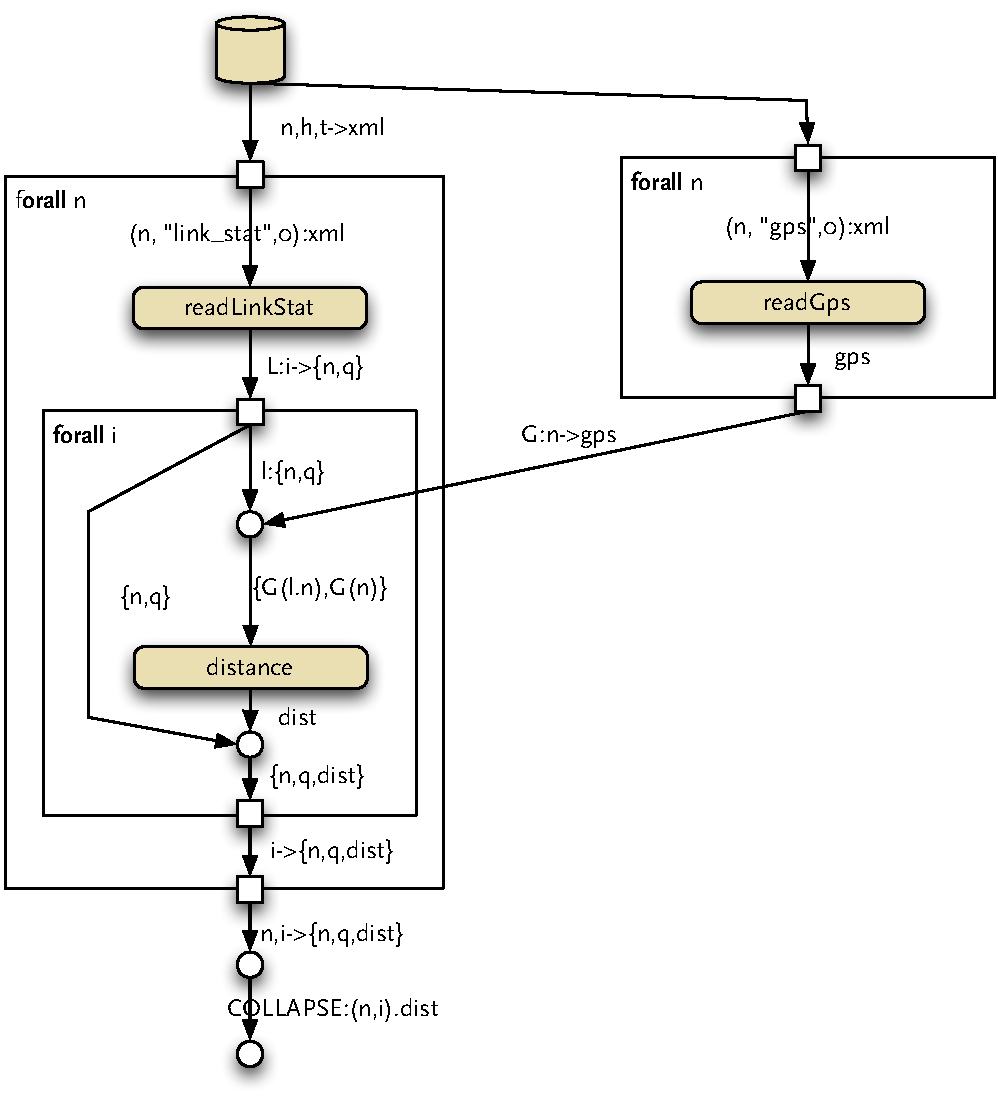
\includegraphics[width=\linewidth]{figures/link_distances_composition}
    \caption{Link distances composition}%
    \label{fig:link_distances_composition}%
  \end{minipage}
\end{figure}

Examples taken from experiments with wireless mesh networks, the experiment pictured in Fig.~\ref{fig:example_analysis_data}. The gps coordinates of two wireless nodes are siblings with the experiment time as closest common ancestor. The gps coordinates of two wireless nodes that form a link are siblings to the link quality of that link with the link as closest common ancestor; further ancestors are the nodes of the link and the experiment time.

Fig.~\ref{fig:seismo_bus_composition} and Fig.~\ref{fig:link_distances_composition} examples for the analysis of HWL ClickWatch data. These activity diagrams choreograph analysis steps (activities). Both are supposed to be performed on HWL ClickWatch data. This is are information graphs (trees). In those nodes have handlers and handlers have XML values at different points in time: hence n, h, t, xml as starting information graph. XML values are part of the information graph.

\subsection{Applications}
\subsection{General}
The described concepts of APD, information and analysis are not new and performed in many fields. What is new is the notion of traces. In complex analysis scenarios traces allow to find siblings and common ancestors, which put the results and intermediate results of an analysis in relation. With other words traces increase the information content of an analysis information graph.

In scenarios, where heterogenous data is produced and analyzed, different types of data is usually analyzed in different analysis steps, threads of analysis steps aggregate the different types of data with each other, and with each further analysis step the created results represent information on increasingly higher levels of abstraction. In such scenarios, it is not trivial to identify all ancestors and siblings of a resulting APD. The semantic for the type of a result is clear, but the semantic of a specific result (the trace of an APD) is not.

\subsection{WMN/WSN}
An example from WMN/WSN. In WMN/WSN experiment scenarios we have a large number of similar (or identical) data sources: the nodes of the network. But each node produces a large number of different APDs. Different sensors, protocol entities, etc. produce all different data. Analysis in this context means that for the different data types on each of the identical nodes different threads of analysis steps are applied. The results are many and complex information graphs that cover different aspects of the network. Trace based knowledge about ancestors and siblings becomes key. 

Why is it key to identify siblings? The seismo sensors in a 100 node network produce different (about 300 in HWL) time signals: one might want to compare the time signals of nodes that are geographically close to each other. Close geographic positions are common ancestors for the time signals. The nodes form links (knowledge about links is a analysis result): it is important to compare the characteristic (analysis result) of one node to the characteristic of linked nodes. Here, nodes are ancestors of the characteristics; the nodes in a link have common ancestors (the links). Looking at a the characteristics of a link or a route (connected links), it is important to identify the characteristics of all nodes in the link or the route. Looking at the time signal of one sensor, one might want to see the time signals of other sensors of that node, or nodes that have links to the node, or nodes in close proximity. Looking at a sensor reading, one might want to see node characteristics recorded at a point in time close to the time of the sensor reading. Etc. etc. etc.



\section{A Framework for Analysis with Traces}\label{sec:framework}

\subsection{Requirements}
\begin{itemize}

\item Large number of data. Information graphs must be scalable. This means that APDs must be indexed somehow to access distance subgraphs efficiently. This is also true for final and intermediate results.

\end{itemize}
\section{Related Work}\label{sec:related_work}

\section{Conclusions}\label{sec:conclusions}


\bibliography{bibliography}

\end{document}
